\documentclass[25pt, a0paper, landscape, blockverticalspace=1cm]{tikzposter}
%\documentclass[]{beamer}



\title{\parbox{\linewidth}{\centering Rotating Stratified Turbulence
}}
\author{Dante Buhl, Pascale Garaud, Hongyun Wang}
\date{April 29, 2025}
\institute{University of California Santa Cruz}
\usetheme{Default}
\usecolorstyle{Default}
\usecolorpalette{Default}

%% PACKAGES %%
\usepackage[utf8]{inputenc}
\usepackage{amsmath, amssymb, amsthm}
\usepackage{mathtools}
\usepackage[shortlabels]{enumitem}
\usepackage{tikz}
\usepackage{subfig}
\usepackage{verbatim}
\usepackage{enumerate}
\usepackage{graphicx}
\usepackage{bm}

%for positioning nodes
\usetikzlibrary{positioning}
\usepackage[none]{hyphenat}


\begin{document}


\newcommand{\red}{\color{red}}
\newcommand{\wrms}{w_{\text{rms}}}
\newcommand{\bs}[1]{\boldsymbol{#1}}
\newcommand{\tb}[1]{\textbf{#1}}
\newcommand{\bmp}[1]{\begin{minipage}{#1\linewidth}}
\newcommand{\emp}{\end{minipage}}
\newcommand{\R}{\mathbb{R}}
\newcommand{\C}{\mathbb{C}}
\newcommand{\N}{\mathcal{N}}
\newcommand{\K}{\bs{\mathrm{K}}}
\newcommand{\m}{\bs{\mu}_*}
\newcommand{\s}{\bs{\Sigma}_*}
\newcommand{\dt}{\Delta t}
\newcommand{\dx}{\Delta x}
\newcommand{\tr}[1]{\text{Tr}(#1)}
\newcommand{\Tr}[1]{\text{Tr}(#1)}
\newcommand{\Div}{\nabla \cdot}
\renewcommand{\div}{\nabla \cdot}
\newcommand{\Curl}{\nabla \times}
\newcommand{\grad}{\nabla}
\newcommand{\pt}{\partial t}
\newcommand{\pz}{\partial z}
\newcommand{\uvec}{\bs{u}}
\newcommand{\F}{\bs{F}}
\newcommand{\T}{\tilde{T}}
\newcommand{\ez}{\bs{e}_z}
\newcommand{\ex}{\bs{e}_x}
\newcommand{\ey}{\bs{e}_y}
\newcommand{\eo}{\bs{e}_{\bs{\Omega}}}
\newcommand{\ppt}[1]{\frac{\partial #1}{\partial t}}
\newcommand{\DDt}[1]{\frac{D #1}{D t}}
\newcommand{\dd}[2]{\frac{d #1}{d #2}}
\newcommand{\pp}[2]{\frac{\partial #1}{\partial #2}}
\newcommand{\ddz}[1]{\frac{d #1}{d z}}
\newcommand{\ppx}[1]{\frac{\partial #1}{\partial x}}
\newcommand{\ppy}[1]{\frac{\partial #1}{\partial y}}


%% images in corners %%
% need to add UCSC logo
\node [below right=-1cm and 5cm] at (bottomleft |- topright)
{
\includegraphics[width=21cm]{ucsc_logo_2.png}};

%% TITLE AND LOGOS %%
\maketitle

\begin{columns}


%%%%%%%%%%%%%%%%%%%%%%%%%%%%%%%%%%%%%%%%%%%%%%%%%%%%%%%%
\column{0.33}
%%%%%%%%%%%%%%%%%%%%%%%%%%%%%%%%%%%%%%%%%%%%%%%%%%%%%%%%


\block{Abstract}
{
Recent interest in the dynamics of stratified turbulence has led to the
development of new models for quantifying vertical transport of momentum and
buoyancy (Chini {\em et al} 2022, Shah {\em et al} 2024). These models are still
incomplete as they do not yet include all of the relevant dynamics often present
in real physical settings such as rotation and magnetic fields. Here we expand
on prior work by adding rotation. We conduct 3D direct numerical simulations of
rotating, stochastically forced, strongly stratified turbulence ($Fr \ll  1$), and vary the Rossby number. We find that rotation gradually suppresses small-scale 3D motions and therefore inhibits vertical transport as Ro decreases towards Fr. The effect is particularly pronounced within the cores of emergent cyclonic vortices. For sufficiently strong rotation, vertical motions are entirely suppressed.
}


\block{Motivation}
{ 
    % TAKE FROM DFD PRESENTATION
\bmp{.47}
    
    Nonrotating stratified turbulence is characterized by strongly
    anisotropic pancake structures within the flow. 

    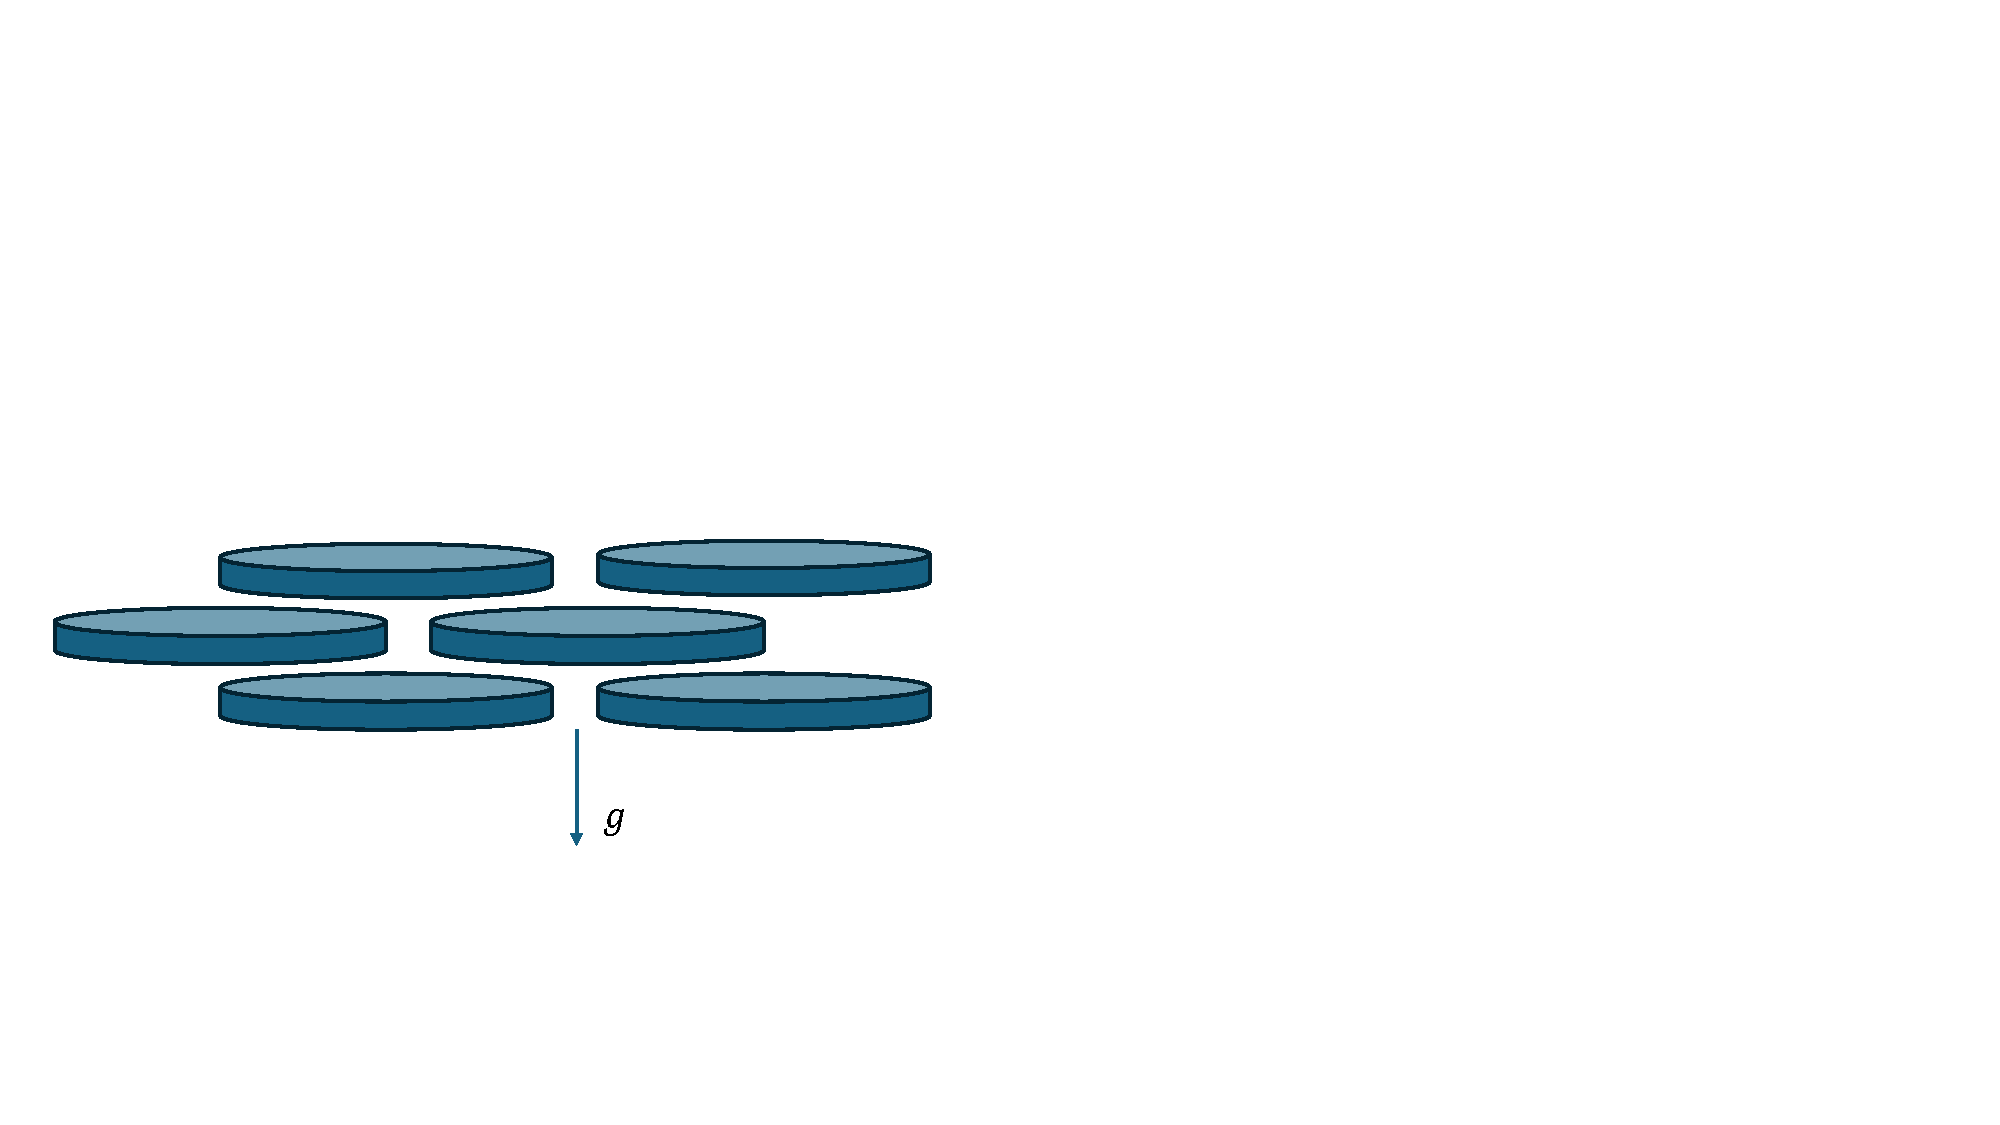
\includegraphics[width=.9\linewidth]{images/pancakes.pdf}
     %end small
\emp
\hfill
\bmp{.47}
    
    Rotation promotes barotropic structures which are invariant along the axis
    of rotation.

    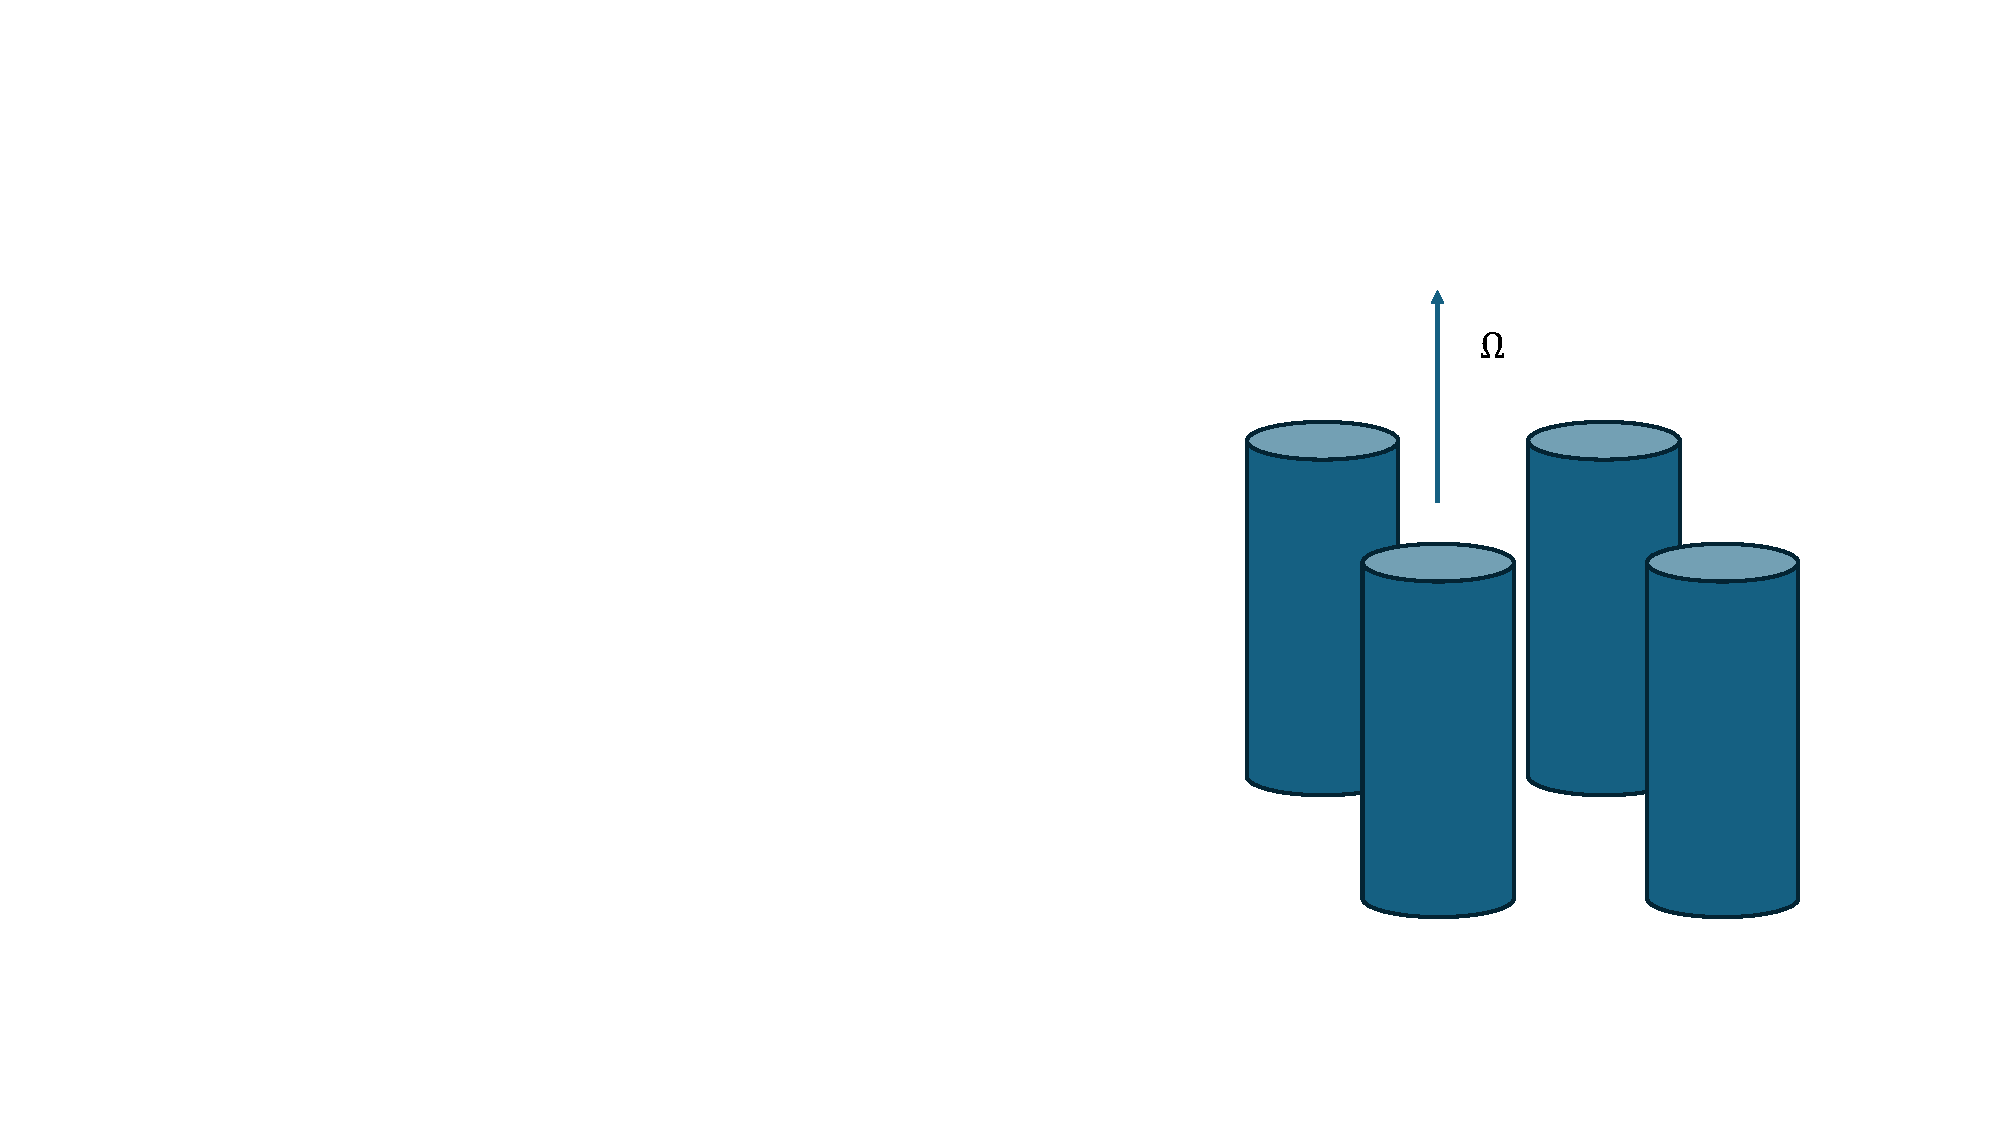
\includegraphics[width=.9\linewidth]{images/cylinders.pdf}
     %end small
\emp
}


\block{The Equations}
{
\begin{align*}
    \DDt{\uvec} + 2\bs{\Omega}\times\uvec = -\frac{1}{\rho}\grad p + \F + \alpha  g T \ez 
    + \nu \grad^2 \uvec\\
    \DDt{T} + w\ddz{\bar{T}} = \kappa \grad^2T\\
    \div{\uvec} = 0
\end{align*}
}


%%%%%%%%%%%%%%%%%%%%%%%%%%%%%%%%%%%%%%%%%%%%%%%%%%%%%%%%
\column{0.33}
%%%%%%%%%%%%%%%%%%%%%%%%%%%%%%%%%%%%%%%%%%%%%%%%%%%%%%%%


\block{Quantitative Results}{
    % start showing data and results. Things to include in this block should be
    % quantitative datas, rms scaling laws with rossby and the such
}

\block{Qualitative Results}{
    % show plots which show qualitative results, things like volume renderings,
    % flow fields, vertical-averaged quantities (top-down)

    % this may be the appropriate section to include the QR code. 
}
%%%%%%%%%%%%%%%%%%%%%%%%%%%%%%%%%%%%%%%%%%%%%%%%%%%%%%%%
\column{0.33}
%%%%%%%%%%%%%%%%%%%%%%%%%%%%%%%%%%%%%%%%%%%%%%%%%%%%%%%%




\block{References}{
}

\block{Acknowledgements}{
    NSF Grant, masters thesis, and other things
}

\end{columns}


\end{document}
